\documentclass[a4paper]{report}
\usepackage{amsmath,amssymb,booktabs,bm,caption,enumerate,float,geometry,graphicx,indentfirst,multirow,setspace,titlesec}
\geometry{left=4.5cm,right=4.5cm,top=4cm,bottom=4cm}
\captionsetup[figure]{labelsep=period}
\captionsetup[table]{labelsep=period}
\begin{document}
	\renewcommand\thesection{\arabic{section}}
	\begin{Large}
		\begin{center}
			\setlength{\baselineskip}{14pt}
			\vspace{1.25cm}
			\rule[0cm]{11.2cm}{0.03em}\\
			\vspace{0.5cm}
			\textsc{UM-SJTU Joint Institute}\\
			\vspace{0.25cm}
			\textsc{Intro to circuits\\(VE215)}
			\vspace{0.3cm}
			\rule[0cm]{11.8cm}{0.05em}
			\vspace{4.9cm}\\
			\textsc{Laboratory Report}
		\end{center}
	\end{Large}
	\vspace{0.85cm}
	\begin{large}
		\begin{center}
			\textsc{Lab 1}
			\vspace{1em}\\
			\textsc{Op Amp Lab}
		\end{center}
		\vspace{6cm}
	\end{large}
	\begin{tabular}{l l}
	Name: Yihua Liu&ID: 518021910998\\
	Name: Han Fang&ID: 518370910009\\
	Name: Yiteng Cai&ID: 518370910007\\
	&\\
	Date: \today&\\
	\end{tabular}
	\thispagestyle{empty}
	\newpage
	\section{Introduction}
	\subsection{Objectives}
	\begin{enumerate}[i.]
		\item Learn how to build and test a variety of circuits based on LM 741 Op Amp chip: non non-inverting and inverting amplifiers with fixed gain.
		\item Measure the gain of the amplifier and compare it with theoretical calculations.
		\item Determine the saturated output voltage of the amplifier.
	\end{enumerate}
	\subsection{Apparatus \& Theoretical Background}
	Operational amplifiers (Op Amps) are integrated circuits (ICs) used in many applications. In this lab, we will build and study LM741.
	\begin{figure}[H]
		\centering
		\includegraphics[width=0.8\linewidth]{1.jpg}
		\caption{Circuit symbol of a typical op amp.}
	\end{figure}
	In Figure 1, there are:
	\begin{itemize}
		\item Two termin als for input signals: inverting (labeled -) 	and non non-inverting (labeled +)
		\item A terminal for the output signal
		\item Two terminals for the power supply voltages: positive +Vcc and negative –Vcc. (e.g. In this lab lab, set +Vcc = 5V; -Vcc = -5V. )
	\end{itemize}
	
	Accordingly, for LM741 op amp chip you see in reality, the pin numbers are shown in Figure 2:
	\begin{figure}[H]
		\centering
		\includegraphics[width=0.8\linewidth]{2.jpg}
		\caption{Pin numbers for LM 741 op amp.}
	\end{figure}
	Note:
	\begin{itemize}
		\item Pin \#8 is not connected; pins \#1 and \#5 are not used in this lab.
		\item We should not mistake the connections of input signals (\#2 labeled – and \#3 labeled +) for the connections to the power supply (\#4 for -Vcc and \#7 for +Vcc).
		\item We should make sure connect the grounds of oscilloscope, function generator and DC source together.
	\end{itemize}
	
	The amplifier circuits are characterized by their gain values. The voltage gain is the ratio of output voltage to the input voltage in the circuit:
	\begin{equation}
	\rm{Voltage\ Gain=\dfrac{Output\ Voltage}{Input\ Voltage}}
	\end{equation}
	
	In the lab, we can use oscilloscope to measure the input and output peak-to-peak (ppk) amplitudes of the signals through two channels at the same time.
	\begin{figure}[H]
		\centering
		\includegraphics[width=0.8\linewidth]{3.jpg}
		\caption{Inverting amplifier.}
	\end{figure}
	For inverting amplifier, the theoretical gain should be:
	\begin{equation}
	\rm{Gain=\dfrac{V_{output}}{V_S}}=1+\dfrac{R_F}{R_A}
	\end{equation}
	
	Apart from the DC source we are already familiar with in Lab 1, we are going to use function generator and oscilloscope this time.
	
	Figure 4 shows the main buttons of the function generator we would use:
	\begin{figure}[H]
		\centering
		\includegraphics[width=1\linewidth]{4.jpg}
		\caption{Function generator.}
	\end{figure}
	\begin{itemize}
		\item “Parameter”: to change the amplitude, frequency of wave to generate.\\*Note: The amplitude here equals to half of the pp value. (i.e. If we set a wave whose amplitude is 100mV, the measured pp value would be 200 Vpp.) pp means peak to peak value.
		\item “1”/“2”: to switch on the channel.
	\end{itemize}
	\begin{figure}[H]
		\centering
		\includegraphics[width=1\linewidth]{5.jpg}
		\caption{Oscilloscope.}
	\end{figure}
	\begin{itemize}
		\item “Auto scale”: to automatically achieve an output on the screen with proper scale.
		\item “Meas”: to turn on the measurement of the wave.
		\item “1”/”2”: to show or hide the wave you detecting through channel 1 or 2.
	\end{itemize}
	\section{Measurement}
	\subsection{Non-inverting amplifier}
	\begin{enumerate}[1.]
		\item Build the circuit according to the figure below below referring to Figure 2, $R_F=100\Omega$, $R_A=50\Omega$. Use the power supply to provide +Vcc = +5V and -Vcc = -5V to the op amp. Use the COM port on the power supply as the ground in the schematic.
		\begin{figure}[H]
			\centering
			\includegraphics[width=1\linewidth]{6.jpg}
			\caption{Non-inverting amplifier.}
		\end{figure}
		\item Use the function generator to generate a sine wave, and use it as the input voltage ($v_i$ in Figure 6). Set the initial amplitude of the sine wave to 0.1 Vpp . Use the oscilloscope to measure the output voltage ($v_o$ in Figure 6).
		\item Increase the input voltage by 0.1 Vpp each time and record the corresponding output until the output voltage is saturate, which means the output voltage is not increasing any more as the input voltage increases.
	\end{enumerate}
	The obtained data is presented in Table 1, 2, and 3.
	\subsection{Inverting amplifier}
	\begin{enumerate}[1.]
		\item Build the circuit according to Figure 7 referring to Figure 2, $R_F=100\Omega$, $R_A=50\Omega$. Use the power supp ly to provide +Vcc = +5V and -Vcc = -5V to the op amp. Use the COM port on the power supply as the ground in the schematic.
		\begin{figure}[H]
			\centering
			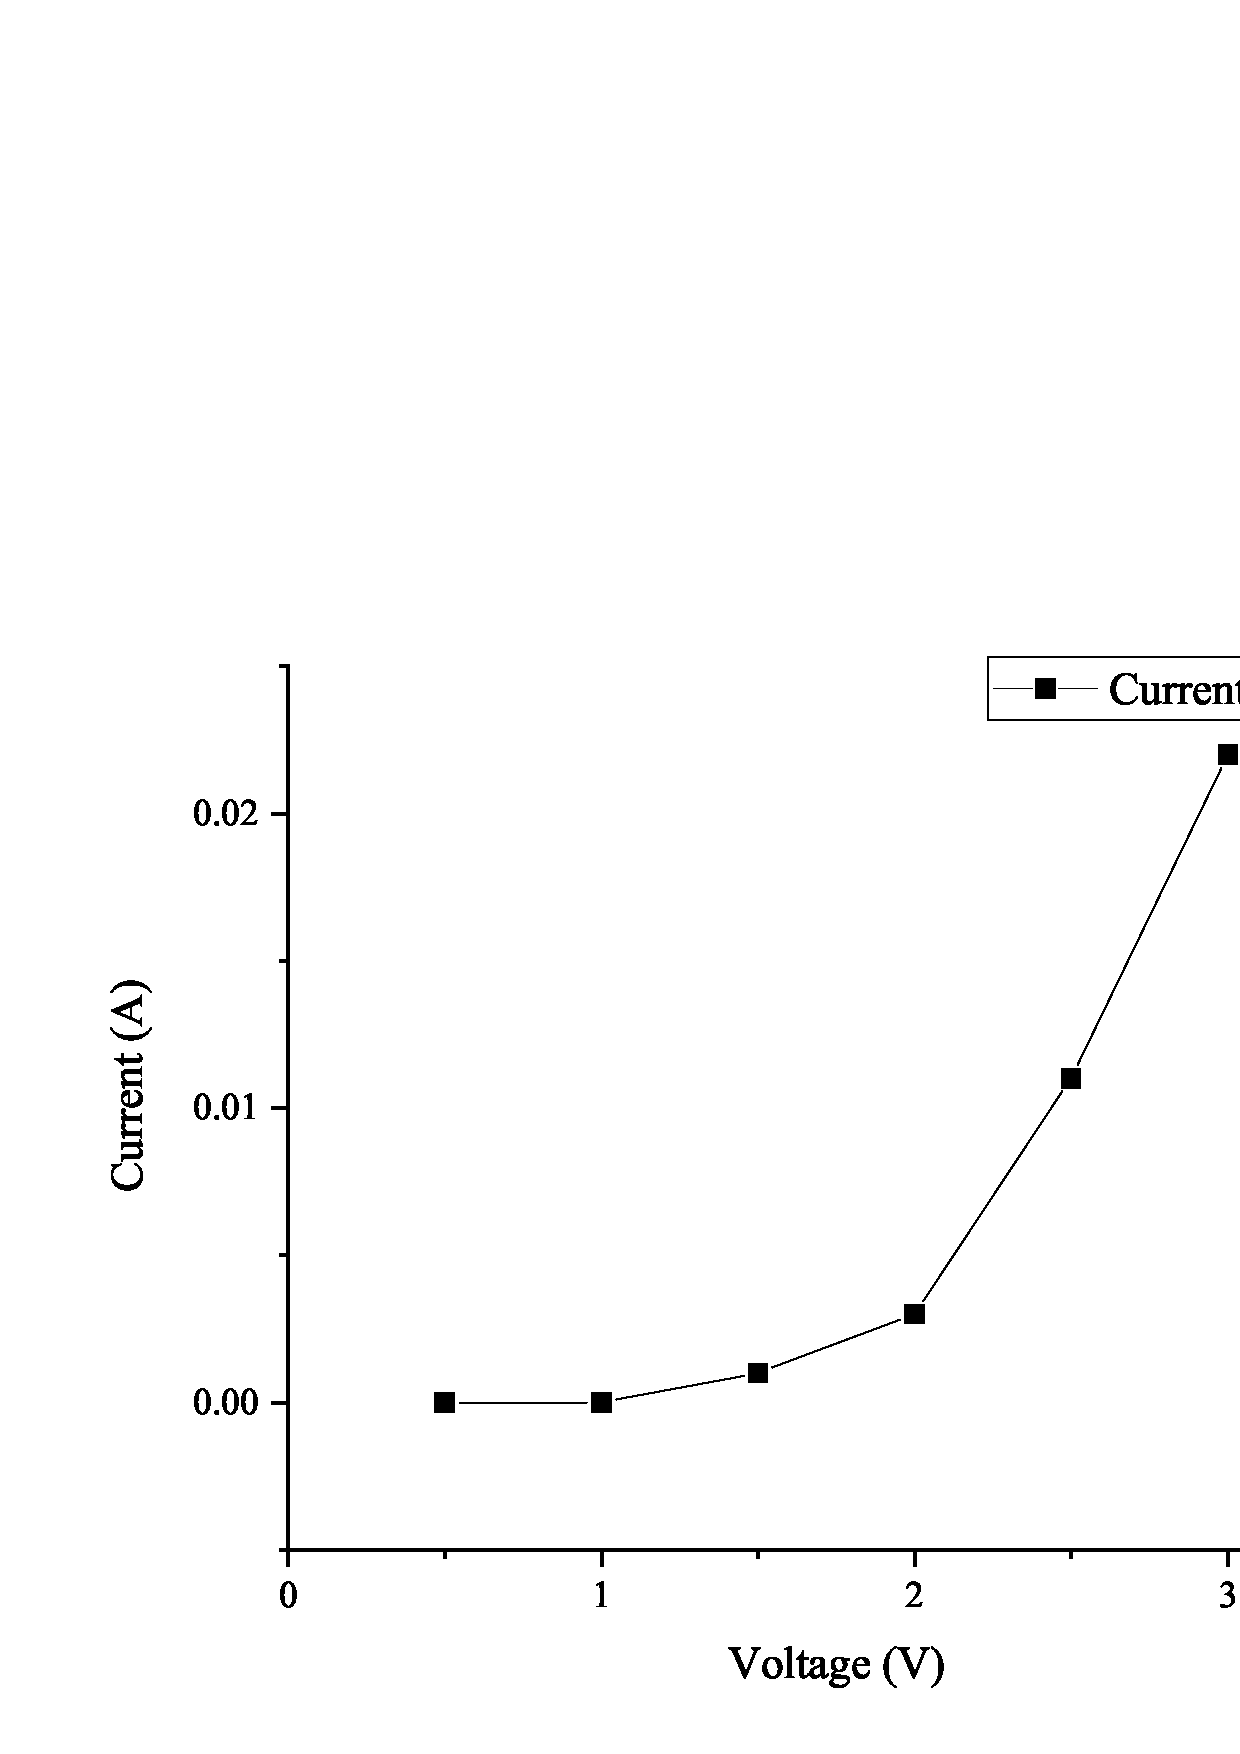
\includegraphics[width=1\linewidth]{7.jpg}
			\caption{Inverting amplifier.}
		\end{figure}
		\item Use the function generator to generate a sine wave, and use it as the input voltage ($v_i$ in Figure 7). Set the initial amplitude of the sine wave to 0.1Vpp. Use the oscilloscope to measure the output voltage ($v_0$ in Figure 7).
		\item Increase the input voltage by 0.1Vpp each time and record the corresponding output until the output voltage is saturate, which means the output voltage is not increasing any more as the input voltage increases.
	\end{enumerate}
	The obtained data is presented in Table 4, 5, and 6.
	\section{Results \& Calculations}
	\subsection{Non-inverting amplifier}
	\begin{table}[H]
		\centering
		\begin{tabular}{|c|c|}
			\hline
			$R_1[\Omega]$&49.9\\
			\hline
			$R_f[\Omega]$&99.9\\
			\hline
		\end{tabular}
		\caption{The resistances of the two resistors we use to build the circuit.}
	\end{table}
	\begin{table}[H]
		\centering
		\begin{tabular}{|c|c|}
			\hline
			$+V_{cc}[\rm{V}]$&5.00\\
			\hline
			$-V_{cc}[\rm{V}]$&-5.00\\
			\hline
		\end{tabular}
		\caption{The voltage supplied to the op amp.}
	\end{table}
	\begin{table}[H]
		\centering
		\begin{tabular}{|c|c|}
			\hline
			$V_{pp(in)}[\rm{V}]$&$V_{pp(out)}[\rm{V}]$\\
			\hline
			0.1000&0.34\\
			\hline
			0.2000&0.64\\
			\hline
			0.3000&0.95\\
			\hline
			0.4000&1.25\\
			\hline
			0.5000&1.54\\
			\hline
			0.6000&1.83\\
			\hline
			0.7000&2.19\\
			\hline
			0.8000&2.49\\
			\hline
			0.9000&2.81\\
			\hline
			1.000&3.12\\
			\hline
		\end{tabular}
		\caption{The input/output relationship.}
	\end{table}
	By Table 3, we can plot the relation between the input voltage and the output voltage ($v_{pp(out)}$ versus $v_{pp(in)}$) in Figure 8.
	\begin{figure}[H]
		\centering
		\includegraphics[width=1\linewidth]{8.eps}
		\caption{The relation between the input voltage and the output voltage ($v_{pp(out)}$ versus $v_{pp(in)}$).}
	\end{figure}
	Using Eq.(1), we can derive the relation between the gain and the input as is shown in Table 4:
	\begin{table}[H]
		\centering
		\begin{tabular}{|c|c|}
			\hline
			$V_{pp(in)}[\rm{V}]$&Gain\\
			\hline
			0.1000&3.4\\
			\hline
			0.2000&3.2\\
			\hline
			0.3000&3.2\\
			\hline
			0.4000&3.13\\
			\hline
			0.5000&3.08\\
			\hline
			0.6000&3.05\\
			\hline
			0.7000&3.13\\
			\hline
			0.8000&3.11\\
			\hline
			0.9000&3.12\\
			\hline
			1.000&3.12\\
			\hline
		\end{tabular}
		\caption{The relation between the input voltage and the output voltage ($v_{pp(out)}$ versus $v_{pp(in)}$).}
	\end{table}
	By Table 4, we can plot the relation between the gain and the input (gain versus $v_{pp(in)}$) in Figure 9.
	\begin{figure}[H]
		\centering
		\includegraphics[width=1\linewidth]{9.eps}
		\caption{The relation between the gain and the input (gain versus $v_{pp(in)}$).}
	\end{figure}
	Using Eq.(2) and Table 1, we can calculate the theoretically expected gain is:
	\begin{equation*}
	\rm{Expected\ Gain}=1+\dfrac{R_F}{R_A}=1+\dfrac{99.9}{49.9}=3.00
	\end{equation*}
	Then, the relative error found by
	\begin{equation*}
	\delta=\rm{\dfrac{Measured\ Gain-Expected\ Gain}{Expected\ Gain}}\times100\%
	\end{equation*}	
	for each value of input is:
	\begin{table}[H]
		\centering
		\begin{tabular}{|c|c|}
			\hline
			$V_{pp(in)}[\rm{V}]$&Relative Error $\delta$\\
			\hline
			0.1000&13\%\\
			\hline
			0.2000&6.6\%\\
			\hline
			0.3000&5.5\%\\
			\hline
			0.4000&4.1\%\\
			\hline
			0.5000&2.6\%\\
			\hline
			0.6000&1.6\%\\
			\hline
			0.7000&4.2\%\\
			\hline
			0.8000&3.8\%\\
			\hline
			0.9000&4.0\%\\
			\hline
			1.000&3.9\%\\
			\hline
		\end{tabular}
		\caption{The relation between the input voltage and relative error of gains $\delta$ ($\delta$ versus $v_{pp(in)}$).}
	\end{table}
	\subsection{Inverting amplifier}
	\begin{table}[H]
		\centering
		\begin{tabular}{|c|c|}
			\hline
			$R_1[\Omega]$&49.9\\
			\hline
			$R_f[\Omega]$&99.9\\
			\hline
		\end{tabular}
		\caption{The resistances of the two resistors we use to build the circuit.}
	\end{table}
	\begin{table}[H]
		\centering
		\begin{tabular}{|c|c|}
			\hline
			$+V_{cc}[\rm{V}]$&5.00\\
			\hline
			$-V_{cc}[\rm{V}]$&-5.00\\
			\hline
		\end{tabular}
		\caption{The voltage supplied to the op amp.}
	\end{table}
	\begin{table}[H]
		\centering
		\begin{tabular}{|c|c|}
			\hline
			$V_{pp(in)}[\rm{V}]$&$V_{pp(out)}[\rm{V}]$\\
			\hline
			0.1000&0.24\\
			\hline
			0.2000&0.46\\
			\hline
			0.3000&0.65\\
			\hline
			0.4000&0.84\\
			\hline
			0.5000&1.05\\
			\hline
			0.6000&1.25\\
			\hline
			0.7000&1.46\\
			\hline
			0.8000&1.64\\
			\hline
			0.9000&1.83\\
			\hline
			1.000&2.01\\
			\hline
		\end{tabular}
		\caption{The input/output relationship.}
	\end{table}
	By Table 8, we can plot the relation between the input voltage and the output voltage ($v_{pp(out)}$ versus $v_{pp(in)}$) in Figure 10.
	\begin{figure}[H]
		\centering
		\includegraphics[width=1\linewidth]{10.eps}
		\caption{The relation between the input voltage and the output voltage ($v_{pp(out)}$ versus $v_{pp(in)}$).}
	\end{figure}
	Using Eq.(1), we can derive the relation between the gain and the input as is shown in Table 9:
	\begin{table}[H]
		\centering
		\begin{tabular}{|c|c|}
			\hline
			$V_{pp(in)}[\rm{V}]$&Gain\\
			\hline
			0.1000&2.4\\
			\hline
			0.2000&2.3\\
			\hline
			0.3000&2.2\\
			\hline
			0.4000&2.1\\
			\hline
			0.5000&2.10\\
			\hline
			0.6000&2.08\\
			\hline
			0.7000&2.09\\
			\hline
			0.8000&2.05\\
			\hline
			0.9000&2.03\\
			\hline
			1.000&2.01\\
			\hline
		\end{tabular}
		\caption{The relation between the input voltage and the output voltage ($v_{pp(out)}$ versus $v_{pp(in)}$).}
	\end{table}
	By Table 9, we can plot the relation between the gain and the input (gain versus $v_{pp(in)}$) in Figure 11.
	\begin{figure}[H]
		\centering
		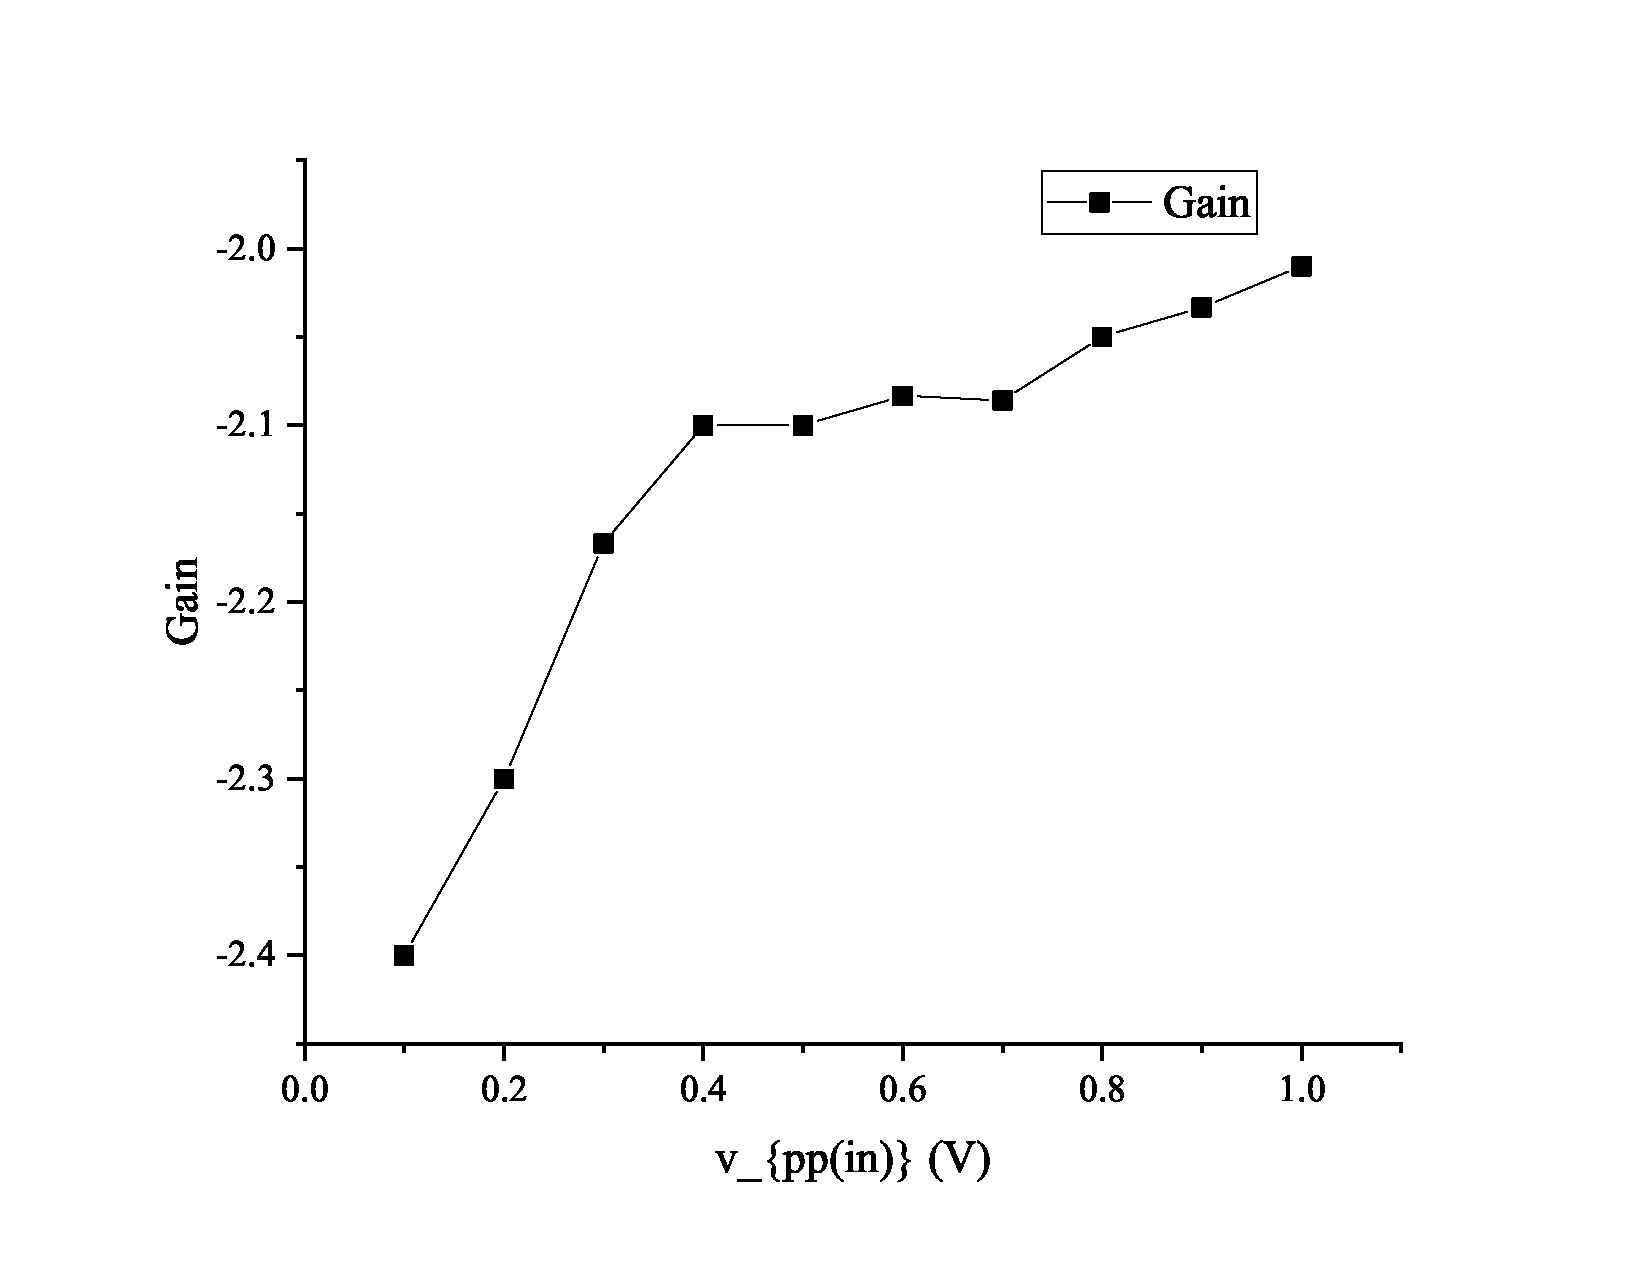
\includegraphics[width=1\linewidth]{11.eps}
		\caption{The relation between the gain and the input (gain versus $v_{pp(in)}$).}
	\end{figure}
	Using Eq.(2) and Table 6, we can calculate the theoretically expected gain is:
	\begin{equation*}
	\rm{Expected\ Gain}=-\dfrac{R_F}{R_A}=-\dfrac{99.9}{49.9}=-2.00
	\end{equation*}
	Then, the relative error found by
	\begin{equation*}
	\delta=\rm{\dfrac{Measured\ Gain-Expected\ Gain}{Expected\ Gain}}\times100\%
	\end{equation*}	
	for each value of input is:
	\begin{table}[H]
		\centering
		\begin{tabular}{|c|c|}
			\hline
			$V_{pp(in)}[\rm{V}]$&Relative Error $\delta$\\
			\hline
			0.1000&20\%\\
			\hline
			0.2000&15\%\\
			\hline
			0.3000&8.2\%\\
			\hline
			0.4000&5.0\%\\
			\hline
			0.5000&5.0\%\\
			\hline
			0.6000&4.1\%\\
			\hline
			0.7000&4.2\%\\
			\hline
			0.8000&2.4\%\\
			\hline
			0.9000&1.6\%\\
			\hline
			1.000&0.40\%\\
			\hline
		\end{tabular}
		\caption{The relation between the input voltage and relative error of gains $\delta$ ($\delta$ versus $v_{pp(in)}$).}
	\end{table}
	\section{Conclusions and Discussion}
	In this experiment, we managed to verify the non-inverting amplifier and inverting amplifier with fixed gain, plotting the relation between the input voltage, the output voltage, and the gain. Besides, we studied the saturated output voltage of the amplifier. Most of the data and the corresponding graphs are generally applicable in accordance with our expectation, but some unexpected errors also occurred.
	
	When the input voltage is high enough, the expected gain is very closed to the measured gain. However, when the input voltage is low, the expected gain is very different from the measured gain. One of the causes of the error is that the unknown mechanism of the wire and the machine we used in the experiment that only works properly when they are matched correspondingly, because these components automatically reduplicate the output voltage for a range of 2 times to even 10 times. Besides, other uncertainties may come from the hand operation on the oscilloscope and the resistance of resistors, since small variation of them leads to great difference of the relative error of the gains.
	
	Last but not least, we learned the usage of the function generator and the oscilloscope for measuring the output voltage, which helps us further develop knowledge of electric circuits.
	\vspace{10cm}
	\section*{Data Sheet}
\end{document}